\documentclass[11pt]{scrartcl}
\usepackage{algorithm}
\usepackage[noend]{algpseudocode}
\usepackage{geometry}
\usepackage{fancyhdr}
\usepackage{tikz}
\pagestyle{fancy}
\rhead{\bfseries Riccardo Salvalaggio, Lorenzo Scarlino}

\geometry{a4paper, top=3cm, bottom=3cm, left=2cm, right=2cm}

%opening
\title{Algorithm Design Exercise Sheet 2}
\author{Riccardo Salvalaggio 1750157 $\&$ Lorenzo Scarlino 1761016}
\subtitle{Course of Engineering in Computer Science, Academic Year 2020/2021}

\begin{document}

\maketitle

\begin{abstract}

\end{abstract}
\newpage
\section{Exercise 1.}
\subsection{Exercise 1.1}
$L_e$ = $\sum_{h \in H_e}x_e$$_h$ $\forall$ e$\in$E\\ 
L = max$_e$$_\in$$_E$$L_e$\\
\textbf{ILP Formulation:}\\
min L\\
s.t.\\
1. $x_e$$_h$ $\in$ $\{$0,1$\}$ $\forall$ e$\in$E,$\forall$ h$\in$H$_e$\Comment{x=1 if elf e visits house h, 0 otherwise}\\
2. $x_e$$_h$ = 0 $\forall$ e$\in$E, $\forall$ h $\notin$ $H_e$\Comment{x=0 if elf e is not able to visit house h}\\
3. $\sum_{h}x_e$$_h$ $\leq$ L $\forall$ e$\in$E\Comment{Sum of all houses visited by an elf isn't greater than makespan}\\
4. $|$$\bigcup_{e \in E}$ $\bigcup_{h \in H_e}$ $x_e$$_h$$|$ = $|$H$|$, $x_e$$_h$ = 1\Comment{Cardinality of all houses visited by all elves is cardinality of H}\\
5. $\sum_{e \in E} x_e$$_h$ = 1 $\forall$ h$\in$H\Comment{Each house has to be visited from exactly one elf, once}\\
\textbf{Relaxed LP Formulation:}\\
min L\\
s.t.\\
1. $x_e$$_h$ $\geq 0$ $\forall$ e$\in$E,$\forall$ h$\in$H\\
2. $\sum_{h}x_e$$_h$ $\leq$ L $\forall$ e$\in$E\\
3. $|$$\bigcup_{e \in E}$ $\bigcup_{h \in H_e}$ $x_e$$_h$$|$ = $|$H$|$, $x_e$$_h$ $>$ 0\\
4. $\bigcap_{e \in E}$$\bigcup_{h \in H_e} x_e$$_h$ = 0, $x_e$$_h$ $>$ 0\\
\subsection{Exercise 1.2}
\vspace{-0.3cm}
\newpage
\section{Exercise 2.}
Building all the sleighs is a non-deterministic problem, because the only way to proceed is to try all possible combination of pieces until all the sleighs are built and different between each other. This resolution is practicable in polynomial time only if there is a certifier A(s,t) such that, given a certificate t (possible solution in input) returns "yes" if it is feasible, "no" otherwise . So the problem belongs to NP.\\
For the construction of the sleighs, it is possible to reduce the problem to a Boolean satisfiabilty formulation (SAT). SAT is a NP-complete problem based on propositional logic. Given a CNF (Conjunctive Normal Form) formula, the problem is solved if there exists a variable assignment which returns true.\\
In order to satisfy all Santa's constraints, we need to concatenate several boolean clauses (with AND,OR,NOT operators) which guarantee the correctness and uniqueness of every sleigh. 
Since Santa has a set P of n pieces,by assuming that there are lot of duplicates of each piece, we can choose l$<$n boolean variables which define all different pieces p$\in$P (excluding dupes).\\For each sleigh i, a variable X$_{pk}$ is set to 1 if piece p of category K is used in the costruction of sleigh i, and 0 otherwise and clauses are set in the following way:\\
1. For each category (i.e. bells,frontlight,seat) it can be used at most one piece:
X$_{pk}$$\wedge$$\neg$(X$_{1k}$$\vee...\vee X_{(p-1)k} \vee X_{(p+1)k} \vee....\vee X_{kk}$), k is the number of different elements of category K;\\
2. There must exist at least one piece of color c: all pieces of color c are in $\vee$ between each other
3. Some pieces must be necessarily matched with some other pieces;\\
4. Some pieces are not consistent together with some other pieces;\\
5. There must exist at least j pieces with a specific characteristic;\\
6. There must exist at most j pieces with a specific characteristic;\\
Given these constraints it is possible to construct a Circuit-SAT instance that solves the problem where we have l leafs that denote all the pieces, then pieces under constraints are connected to their boolean clause to ensure integrity; each clause compute and returns a value. At the end this construction tells if the input instance is a feasible one (so it makes circuit compute correct values at each node) and collect it.
Once all combinations have been computed it is possible to check, from the collected ones, if there exists the amount of sleighs required by Santa.
Since Circuit-SAT is NP-Complete (first NP-Complete problem demonstrated), and having proved that our problem is in NP, we can finally say that our problem is NP-Complete.




\newpage
\section{Exercise 3.}
\subsection{Exercise 3.1}
Given the hint, the graph which represent the game G is the following:\\
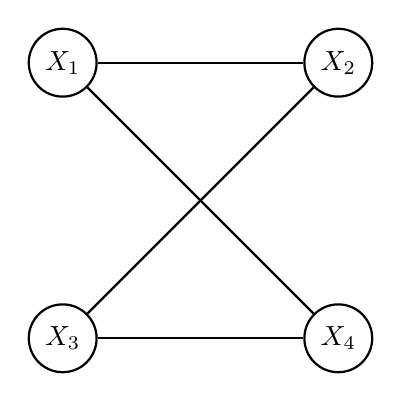
\begin{tikzpicture}[node distance={35mm},thick,main/.style = {draw, circle}] 
\node[main] (1) {$X_1$}; 
\node[main] (2) [right of=1] {$X_2$};
\node[main] (3) [below of=1] {$X_3$};
\node[main] (4) [below of=2] {$X_4$};
\draw (1) to (2);
\draw (2) to (3);
\draw (3) to (4);
\draw (1) to (4);
\end{tikzpicture}
\\
Price of Anarchy is the quantity: $\frac{max_{s \in S} \sum_{i\in N} u_i(s)}{min_{s \in E} \sum_{i\in N} u_i(s)}$.\\
The set of equilibria for the minimum denominator is given by the following CUT($\alpha$): $X_1\gets$ $\{$LEFT$\}$, $X_2\gets$ $\{$LEFT$\}$,$X_3\gets$ $\{$RIGHT$\}$, $X_4\gets$ $\{$RIGHT$\}$.\\
Total payoff of CUT($\alpha$):  U($\alpha$) $\gets$ $\sum_{i \in N} $$\sum_{e \in CUT(\alpha)\cap N_i}{\omega_e}$ = 4.\\
The set of equilibria for the maximum numerator is given by the following CUT($\alpha$): $X_1\gets$ $\{$LEFT$\}$, $X_2\gets$ $\{$RIGHT$\}$,$X_3\gets$ $\{$LEFT$\}$, $X_4\gets$ $\{$RIGHT$\}$.\\
Total payoff of CUT($\alpha$):  U($\alpha$) $\gets$ $\sum_{i \in N} $$\sum_{e \in CUT(\alpha)\cap N_i}{\omega_e}$ = 8.\\
So the Price of Anarchy of game G is PoA(G) = $\frac{8}{4}$ = 2.
\subsection{Exercise 3.2}
In a pure Nash equilibrium, each vertex $v_i$ in the graph G has no interest in changing his status (from LEFT to RIGHT or viceversa), so the total weight of his neighbouring vertices in the cut (i.e. with different status from $v_i$) is at least equal to the total weight of neighbouring vertices which are not in the cut (i.e. with the same status of $v_i$). If this were not the case, the vertex $v_i$ should have an advantage in changing his status, and we could not speak of PNE.\\
By expanding this concept to the entirety of the graph, in any cut game $\Gamma$, in a PNE, the global payoff (total weight in the cut) is at least equal to 2$\cdot$(half the total weight of all edges in the graph) = total weight of the graph (each edge appears twice in the calculation).\\
On the other hand, the maximum global payoff achievable in $\Gamma$ is at most 2$\cdot$(total weight of the graph), that it means that every edge in the graph is in the cut (every vertex has only neighbours with a different status).\\
Thus, the Price of Anarchy of $\Gamma$ is at most:\\
\begin{center}
PoA($\Gamma$) = $\frac{max_{s \in S} \sum_{i\in N} u_i(s)}{min_{s \in E} \sum_{i\in N} u_i(s)}$ = $\frac{2\cdot TotalWeight(\Gamma)}{TotalWeight(\Gamma)}$ = 2.
\end{center}
\section{Exercise 4.}
\subsection{Exercise 4.1}
\vspace{-0.2cm}
\subsection{Exercise 4.2}
\vspace{-0.4cm}
\end{document}
